% The main file. It contains definitions of basic parameters and includes all other parts.

% Meta-data of your thesis (please edit)
\input metadata.tex

% Generate metadata in XMP format for use by the pdfx package
\input xmp.tex

%% Settings for single-side (simplex) printing
% Margins: left 40mm, right 25mm, top and bottom 25mm
% (but beware, LaTeX adds 1in implicitly)
% \documentclass[12pt,a4paper]{report}
% \setlength\textwidth{145mm}
% \setlength\textheight{247mm}
% \setlength\oddsidemargin{15mm}
% \setlength\evensidemargin{15mm}
% \setlength\topmargin{0mm}
% \setlength\headsep{0mm}
% \setlength\headheight{0mm}
% % \openright makes the following text appear on a right-hand page
% \let\openright=\clearpage

%% Settings for two-sided (duplex) printing
% \documentclass[12pt,a4paper,twoside,openright]{report}
% \setlength\textwidth{145mm}
% \setlength\textheight{247mm}
% \setlength\oddsidemargin{14.2mm}
% \setlength\evensidemargin{0mm}
% \setlength\topmargin{0mm}
% \setlength\headsep{0mm}
% \setlength\headheight{0mm}
% \let\openright=\cleardoublepage

%% If the thesis has no printed version, symmetric margins look better
\documentclass[12pt,a4paper]{report}
\setlength\textwidth{145mm}
\setlength\textheight{247mm}
\setlength\oddsidemargin{10mm}
\setlength\evensidemargin{10mm}
\setlength\topmargin{0mm}
\setlength\headsep{0mm}
\setlength\headheight{0mm}
\let\openright=\clearpage

\usepackage{amssymb}
\usepackage{tikz}
\tikzset{vertex/.style={fill=black, circle, minimum size=1pt, inner sep=0.3pt}, label distance=1pt, line width=0.8pt}

\usepackage{caption}
\usepackage{subcaption}
%% Generate PDF/A-2u
\usepackage[a-2u]{pdfx}

%% Prefer Latin Modern fonts
\usepackage{lmodern}
% If we are not using LuaTeX, we need to set up character encoding:
\usepackage{iftex}
\ifpdftex
\usepackage[utf8]{inputenc}
\usepackage[T1]{fontenc}
\usepackage{textcomp}
\fi

%% Further useful packages (included in most LaTeX distributions)
\usepackage{amsmath}        % extensions for typesetting of math
\usepackage{amsfonts}       % math fonts
\usepackage{amsthm}         % theorems, definitions, etc.
\usepackage{bm}             % boldface symbols (\bm)
\usepackage{booktabs}       % improved horizontal lines in tables
\usepackage{caption}        % custom captions of floating objects
\usepackage{dcolumn}        % improved alignment of table columns
\usepackage{floatrow}       % custom float environments
\usepackage{graphicx}       % embedding of pictures
\usepackage{indentfirst}    % indent the first paragraph of a chapter
\usepackage[nopatch=item]{microtype}   % micro-typographic refinement
\usepackage{paralist}       % improved enumerate and itemize
\usepackage[nottoc]{tocbibind} % makes sure that bibliography and the lists
			    % of figures/tables are included in the table
			    % of contents
\usepackage{xcolor}         % typesetting in color
\usepackage{comment}
\usepackage{soul}
\usepackage[utf8]{inputenc}
\DeclareRobustCommand{\comment}[1]{ {\begingroup\sethlcolor{cyan}\hl{(comment:) #1}\endgroup} }

% The hyperref package for clickable links in PDF and also for storing
% metadata to PDF (including the table of contents).
% Most settings are pre-set by the pdfx package.
\hypersetup{unicode}
\hypersetup{breaklinks=true}

% Packages for computer science theses
\usepackage{algpseudocode}  % part of algorithmicx package
\usepackage{algorithm}
\usepackage{fancyvrb}       % improved verbatim environment
\usepackage{listings}       % pretty-printer of source code

\algnewcommand{\algorithmicelseif}{\textbf{else if}}
\algdef{SE}[IF]{If}{EndIf}[1]{\algorithmicif\ #1\ \algorithmicthen}{\algorithmicend\ \algorithmicif}
\algdef{SE}[ELSEIF]{ElsIf}{EndElsIf}[1]{\algorithmicelseif\ #1\ \algorithmicthen}{\algorithmicend\ \algorithmicif}

% You might want to use cleveref for references
% \usepackage{cleveref}

% Set up formatting of bibliography (references to literature)
% Details can be adjusted in macros.tex.
%
% BEWARE: Different fields of research and different university departments
% have their own customs regarding bibliography. Consult the bibliography
% format with your supervisor.
%
% The basic format according to the ISO 690 standard with numbered references
\usepackage[natbib,style=iso-numeric,sorting=none]{biblatex}
% ISO 690 with alphanumeric references (abbreviations of authors' names)
%\usepackage[natbib,style=iso-alphabetic]{biblatex}
% ISO 690 with references Author (year)
%\usepackage[natbib,style=iso-authoryear]{biblatex}
%
% Some fields of research prefer a simple format with numbered references
% (sorting=none tells that bibliography should be listed in citation order)
%\usepackage[natbib,style=numeric,sorting=none]{biblatex}
% Numbered references, but [1,2,3,4,5] is compressed to [1-5]
%\usepackage[natbib,style=numeric-comp,sorting=none]{biblatex}
% A simple format with alphanumeric references:
%\usepackage[natbib,style=alphabetic]{biblatex}

% Load the file with bibliography entries
\addbibresource{bibliography.bib}

% Our definitions of macros (see description inside)
\input macros.tex

%%% Title page and various mandatory informational pages
\begin{document}
\include{title}

%%% A page with automatically generated table of contents of the thesis

\tableofcontents

%%% Each chapter is kept in a separate file
\chapter{Introduction}

The four-color theorem, that every planar graph is four-colorable, was one of the central problems
in graph theory for over a century. Appel and Haken proved it in 1976 \cite{appel_haken_1977} using a computer program.
The proof was controversial because it was the first major theorem to be proved using a computer.
The theorem was later proved in 1997 by Robertson, Sanders, Seymour, and Thomas \cite{ROBERTSON19972},
still using a computer but with more straightforward configurations than Appel and Haken's in several aspects. 

Hadwiger's conjecture \cite{hadwiger_1943} suggests a generalization of the four-color theorem. It is considered one of 
the most challenging problems in graph theory. Before stating the conjecture, we define the notion of a \textit{graph minor}.

\begin{defn}[Minor]
    The $G$ contains a graph $H$ as a \textit{minor} if there exist a system $\{B_v : v \in V(H)\}$ of pairwise disjoint subsets of $V(G)$
    such that:
       \begin{itemize}
           \item For every vertex $v$ from $V(H)$, the subgraph of $G$ induced by vertices $B_v$, denoted $G[B_v]$, is connected.
           \item For every edge $u,v$ in $E(H)$, there is an edge of $G$ with one end in $G[B_u]$ and the other end in $G[B_v]$.
       \end{itemize} 

       We say that the system $\{B_v : v \in V(H)\}$ is a model of $H$ in $G$.
\end{defn}

\begin{conj} [Hadwiger 1943 \cite{hadwiger_1943}]
 For every integer $k \geq 0$, every graph $G$ with no $K_{k+1}$ minor can be colored with $k$ colors.
\end{conj}

Equivalently, it can be stated that every graph with chromatic number at least $k$ contains $K_k$ minor.

It was proved by Hadwiger himself for cases $k \leq 3$. Wagner \cite{wagner_1937} showed that the case $k = 4$ is equivalent to the four-color theorem.
\begin{enumerate}
    \item \textit{Forward direction:} The case $k = 4$ implies the four color theorem since by Wagner \cite{wagner_1937}, every planar graph has no $K_5$ or $K_{3, 3}$ as 
 minors. Hence all planar graphs do not have $K_5$ as minor. Hadwiger's conjecture for case $k = 4$ claims if graph doesn't contain
    $K_5$ as minor, then it is $4$-colorable.
    \item \textit{Reverse direction:} Wagner \cite{wagner_1937} showed that a graph $G$ is $K_5$-minor free if it is obtained by 
clique sums of planar graphs and a Wagner graph $W$, where $W$ is a 3-colorable non-planar graph on eight vertices.
For any two four-colorable graphs, their clique sum is also four-colorable. Hence, the four-color theorem implies Hadwiger's conjecture
for the case $k = 4$.
\end{enumerate}

Robertson, Seymour, and Thomas proved the case $k = 5$ in 1993 \cite{robertson_seymour_1993}, 
where they did not use a computer to prove it. However, they proved that a minimal counter-example to the case $k = 5$ should have 
a vertex whose removal results in a planar graph, reducing the problem to the four-color theorem. The case $k = 6$ is still open, and there are some results in this direction as that of Albar and Gonçalves \cite{albar_goncalves_2013}. 
\begin{thm}
 Every graph with no $K_7$ minor is 8-colorable, and every graph with no $K_8$ minor is 10-colorable.
\end{thm}

Moreover, Kawarabayashi and Toft \cite{Kawarabayashi2005} proved that every 7-chromatic graph has $K_7$ or $K_{4,4}$ as minor.
Bollobás, Catlin, and Erdös \cite{BOLLOBAS1980195} showed that the conjecture is true for almost all graphs using
probabilistic arguments. In general, the cases $k \geq 6$ remain open.
Because of the conjecture's current state, there is interest in a weaker version known as the Linear Hadwiger's Conjecture.

\begin{conj} (Linear Hadwiger's Conjecture)
 There exists a constant $c$ such that, for every $k \geq 0$, every graph with no $K_{k+1}$ minor can be colored with $ck$ colors.
\end{conj}

For more than forty years, the best-known result for the linear version was that every graph with no $K_{t+1}$ minor is $O(t \sqrt{\log t})$-colorable.
This was proved in the 1980s by Kostochka \cite{Kostochka1984} and Thomason \cite{Thomason_1984} independently.
Recently, in 2025, Delcours and Postle \cite{JAMS2025} lowered this bound to $O(k \log \log(k))$.

Holroyd\cite{Holroyd1997} tryied to strengthen Hadwiger’s conjecture by looking specific regions in a graph where a minor of a complete graph is likely to appear, based on the coloring of the region.
Before stating his conjecture, we need to define the concepts of rooted minors and colorful sets.

\begin{defn}[Rooted minor]
    Let $G$ and $H$ be graphs and let $S = \{X_v : v \in V(H)\}$ be a system of distinct vertices of $G$. Then $H$
    is an $S$-rooted minor of $G$ if exists a model $\{B_v : v \in V(H)\}$ of $H$ in $G$ such that for every
    vertex $v \in V(H)$ $X_v \in B_v$.
\end{defn}

\begin{defn}[Chromatic coloring]
    Let $G$ be a graph. The chromatic number of $G$ denoted as $\chi(G)$ is the smallest integer $k$ such that $G$ is 
    properly colored with $k$ colors. We say that a coloring $\mathfrak{C}$ is chromatic coloring of the graph $G$ if 
    it has exactly $\chi(G)$ color classes.
\end{defn}

\begin{defn}[Colorful set]
 For a graph $G$, a set of vertices $S \subseteq V(G)$ is called \textit{colorful} in $G$ if for every chromatic coloring of $G$, $S$ contains at least one 
 vertex from each color of the coloring.
\end{defn}

The colorful sets of the graph are places that are 'hard to color'. Hence, we might hope to find the $K_{t}$ minors rooted in those sets. And this is 
exactly the Halroyd's conjecture.

\begin{conj} (Halroyd's conjecture)
 Let $G$ be a graph with chromatic number $k$, let $S$ be a colorful set in $G$. Then there exists
 a subset $S' \subseteq S$ of size $k$ such that $G$ has an $S'$-rooted $K_k$ minor. 
\end{conj}

\comment{In notes I have: Formulate that the system doesn't matter for complete graphs for colorful sets. 
I am not sure what we wanted to say there}

Holroyd called it the Strong Hadwiger Conjecture because it generalizes Hadwiger's conjecture. If we take $S = V(G)$,
then the Halroyd's conjecture states that there exists an $S' \subseteq S$ of size $k$ such that the graph $G$ has $S'$-rooted $K_k$ minor. 
Since the set $S$ is the all vertices of graph $G$, it means $G$ contains $K_k$ as a minor
which is exactly the statement of Hadwiger's conjecture.

Holroyd himself proved conjecture for cases $k \leq 3$ \cite{Holroyd1997}, and in 2024  the case
$k = 4$ was proved by Martinsson and Steiner \cite{MARTINSSON20241}.

A classical tool in studying Hadwiger's conjecture is the notion of Kempe chains. It was first introduced by Kempe in an attempt
to prove the four-color theorem. Even though his proof was not correct, Kempe chains were shown to be very useful in problems 
related to Hadwiger’s conjecture. They were used for proving the four-color and five-color theorems as well.

\section{Kempe chains}

\begin{defn}[Proper coloring]
    A proper (vertex) coloring of a graph $G$ is a coloring of the vertices of $G$ such that no two adjacent vertices
    share the same color.
\end{defn}

\comment{Should we define proper coloring earlier, and also say that we assume that all colorings are proper? Because
by default we assume it throughout the paper}

\begin{defn}[Kempe chain]
 Let $G$ be a graph with proper coloring. Then for two distinct color classes $i$ and $j$, the Kempe chain 
 in colors $i$ and $j$ is the maximal connected subgraph of $G$ where vertices have only colors of $i$ or $j$.
\end{defn}

\begin{claim}
    \label{colorful_kempe}
    Let $G$ be a graph with proper coloring and let $S$ be a colorful set in $G$. For a color class $i$, let 
    $S_i$ be the set of vertices from $S$ that have color $i$. Then for every distinct color classes $i$ and $j$
    There exists a Kempe chain between some of the vertices of $S_i$ and $S_j$.
\end{claim}
\begin{proof}
    Assume for contradiction that there is no Kempe chain between $S_i$ and $S_j$.  We will show that we can recolor the vertices of $S_i$ with color $j$ and still maintain a proper coloring, contradicting the assumption that $S$ is colorful (since in the new coloring, no vertex of $S$ has color $i$).
    
    \begin{enumerate}
      \item Let $v\in S_i$.
        \begin{itemize}
          \item If $v$ is not contained in any Kempe chain of colors $i$ and $j$.
          \item Otherwise, $v$ lies in some Kempe chain of colors $i$ and $j$.  By our assumption, that Kempe chain contains no vertices of $S_j$ we can switch the colors $i\leftrightarrow j$ along that chain. The resulting coloring is proper, where $v$ now has color $j$.
        \end{itemize}
      \item Repeat this for each vertex of $S_i$.  At each step, properness is maintained, and no vertex of $S_j$ is ever touched (since there are no $i$–$j$ chains reaching $S_j$).  After recoloring all of $S_i$, the colorful set $S$ no longer contains any vertex of color $i$, a contradiction.
    \end{enumerate}
    
    Hence there exists a Kempe chain connecting some vertex in $S_i$ to some vertex in $S_j$.
    \end{proof}
    
We can observe that the vertices of colorful sets from Halroyd's conjecture must be connected by Kempe chains.
Suppose, for contradiction, that there exist two vertices  $u, v$ in a colorful set, colored  $i$ and  $j$ respectively,
but no Kempe chain of colors  $i$ and  $j$ connects them.
Then, consider the Kempe chain of colors  $i$ and  $j$ that contains  $u$. Swapping the colors within this chain—replacing every  $i$ with  $j$ and vice versa—produces a new proper coloring of the graph.
However, this would result in  $u$ taking the same color as  $v$, contradicting the assumption that the set is colorful.
Thus, every pair of vertices in a colorful set must be connected by a Kempe chain.

Since Hadwiger's conjecture is difficult to prove in general, it is interesting to study it for specific classes of graphs.
Hadwiger suggested looking into the graphs with a bounded number of optimal colorings \cite{hadwiger_1943}, 
one particular class is the uniquely optimally colorable graphs.

\begin{claim}
 Let $G$ be a uniquely $k$-colorable graph with colors $\{1, 2, \dots, k\}$ Let $v_1, v_2, \dots, v_k$ be differently colored vertices of the graph $G$, 
 where $v_i$ is has color $i$.
 Then there are Kempe chains between all pairs of $v_i$ and $v_j$ from $\{v_1, v_2, \dots, v_k\}$.
\end{claim}


\begin{proof}
    Let $S := \{v_1, v_2, \dots, v_k\}$, then $S$ is a colorful set. By the claim \ref{colorful_kempe} for every distinct color classes
    $i$ and $j$ there exists a Kempe chain between $S_i$ and $S_j$. Since each color appears only once in $S$, we have that
    each $S_i$ has size of 1. Hence, there is a Kempe chain between each distinct pair of the vertices of the colorful set.
\end{proof}

This claim suggests a question: whether the existence of the Kempe chains forces an existence of $K_k$ minor rooted at
$\{v_1, v_2, \dots, v_k\}$.

Kriesell proved the Hadwiger’s conjecture for uniquely $k$-colorable graphs where $k \leq 10$ \cite{Kriesell2021}, if the graph is antitriangle-free \cite{Kriesell2017}.
Moreover, with Mohr, they proved it is true for line graphs \cite{Kriesell2019}.

\section{Rooted minors}
One of the central problems in Graph Theory is to find a minor in a given graph. There has been significant progress 
in this direction, one of which is the structure theorem of Robertson and Seymour, which says that if a graph $G$ does not have
$K_t$ minor, then $G$ is ``almost embeddable'' on a surface of low Euler genus relative to $t$ \cite{RobertsonSeymourGM16}.
This result was developed as part of their proof of Wagner's Conjecture—now known as the Robertson–Seymour Theorem
—which says that the class of finite undirected graphs is well-quasi-ordered under the graph minor relation.
In the proof, they use the following theorems, which are proved in \cite{RobertsonSeymourGM20}

\begin{thm}
 let $G$ be a 3-connected graph and let $v_1, v_2, v_3$ be three distinct vertices. Then either $G$ has 
 five connected disjoint subgraphs $X_1, X_2, \dots, X_5$ such that $X_i$ contains $v_i$ for every $i = 1,2,3$
 and for every $j = 4,5$ $X_j$ has neighbour in each $X_i$ for all $i = 1,2,3$ or $G$ is planar such that $v_1, v_2, v_3$ are on boundary.
\end{thm}

\begin{thm}
 Let $G$ be a 4-connected graph and $v_1, v_2, v_3, v_4$ be four distinct vertices. Then either $G$ has $K_4$ minor rooted
 at $\{v_1, v_2, v_3, v_4\}$ or $G$ is planar such that $v_1, v_2, v_3, v_4$ are on the boundary.
\end{thm}

Those two results were the starting points for rooted minor problems. 
\newline
It turns out that rooted minors are not only
useful for the proof of Graph Minor theorem, but also for some structure theorems which are used to prove some existence
of graph minor, some of which are presented below:

Robertson, Seymour, and Thomas \cite{robertson_seymour_1993} used rooted $K_4$–minors to prove the case $k=5$ of Hadwiger's conjecture.
Kawarabayashi and Toft \cite{Kawarabayashi2005} used rooted minors to prove that every 7-chromatic graph has $K_7$ or $K_{4,4}$ as minor.

In graphs embedded on surfaces, the concept of a rooted minor extends naturally to problems involving
face covers. A recent paper \cite{Fiorini2025} shows that in a 3-connected
graph embedded in a surface of Euler genus $g$, if the graph has no rooted $K_{2,t}$ minor,
then there exists a face cover whose size is bounded by a function of $g$ and $t$. 
In the planar case, they got $O(t^4)$ upper bound, which improved the result of Böhme and Mohar~\cite{BOHME2002291}.

\subsection*{Kempe chains and rooted minors}
Usually, in the context of Hadwiger's conjecture, only clique minors were considered. However, Kriesell and Mohr \cite{matthias_2022} considered
the following question, which does not necessarily look for clique minors. Let $G$ be a graph with a proper coloring
$\mathfrak{C}$, let $k = |\mathfrak{C}|$, and let $v_1, ..., v_{k}$ be a vertex set of $G$ with different colors.
Then, there is a system of Kempe chains for some pairs $(v_i, v_j)$.
They examined whether there is a rooted minor $H$ of $G$ on vertices $v_1, ..., v_{k}$, where $H$ has edges between 
$v_i, v_j$ if and only if there is a Kempe chain between $v_i$ and $v_j$ in $G$.

The answer to this question is affirmative for the case $k \leq 4$. For $k = 5$,
it holds for graphs with at most six edges but remains open in general.
The case $k = 6$ is also open, while counterexamples exist for $k \geq 7$.

In this paper, we investigate properties of minimal counterexample graphs for the case $k = 5$.
Additionally, we perform a computational enumeration for $k = 6$, examining all graphs with at most sixteen vertices.
Our results show that the answer remains positive for all graphs in this range.


\chapter{Preliminaries}

In this chapter, we will present definitions and primary results from the paper of 
Kriesell and Mohr \cite{matthias_2022}, which we will use to build up our investigations.

They introduced the concept of \textit{routing graphs} to more formally characterize the problem from the previous chapter, as we saw. 
First, let us define the transversal of a set partition, and then we can define the routing graph.

\begin{defn}[Transversal of a partition]
 A (minimal) transversal of a partition is a set containing exactly one
 element from each partition member and nothing else.
\end{defn}

\begin{example}
 Coloring $\mathfrak{C}$ of a graph partitions its vertices into color classes. 
 A transversal $T$ of this partition would contain exactly one vertex of each color from $\mathfrak{C}$.
\end{example}

\begin{defn}[Routing Graph]
Let $\mathfrak{C}$ be a coloring of graph $G$, let $T$ be the transversal of coloring $\mathfrak{C}$, 
then the routing graph $H(G, \mathfrak{C}, T)$ is the graph with vertex set $T$,
where for every pair of vertices $u,v$ from $T$, an edge $(u,v)$ exists if and only if
there is a Kempe chain between $u$ and $v$ in $G$.
\end{defn}

Now, we can define the problem in a more compact way, which is as follows:

Which graphs $H$ have the property that, if $H$ is a
routing graph of some graph $G$ with coloring $\mathfrak{C}$ and a transversal $T$, then G
has $H$ as $T$-rooted minor? We say those graphs are \textit{KM-forcing}.

\section{KM-forcing graphs}

\begin{defn}[KM-forcing]
 A graph $H$ is KM-forcing if for every graph $G$, coloring $\mathfrak{C}$ and transversal $T$
 such that $H$ is isomorphic to the routing graph $H(G, \mathfrak{C}, T)$, graph $G$ has $H$ as $T$-rooted minor.
\end{defn}

\begin{rem}
    The term \emph{KM-forcing} can be interpreted in two ways: as \emph{Kriesell–Mohr forcing} or as \emph{Kempe chain rooted minor forcing}. We leave the choice of interpretation to the reader’s imagination.
\end{rem}

\begin{example}
    $K_1$ is KM-forcing. If $K_1$ is a routing graph $H(G, \mathfrak{C}, T)$, then $|T| = 1$, and $G$
can be colored with only one color; hence, it has no Kempe chains to other colored vertices, and $K_1$ is a rooted minor of $G$.
\end{example}

\begin{example}
 The complete graph $K_2$ is KM-forcing. 
 For any graph $G$ with coloring $\mathfrak{C}$ and transversal $T = \{u,v\}$ where the routing graph $H(G, \mathfrak{C}, T)$ is
 isomorphic to $K_2$, by definition there exists a Kempe chain between $u$ and $v$ in $G$. 
 Contracting all internal vertices of this chain while keeping $u$ and $v$ results in an edge $(u, v)$. In the contracted graph of $G$,
 removing all unnecessary edges and vertices would result in $K_2$ as a rooted minor of $G$.
\end{example}

We will list several results from \cite{matthias_2022}, which capture properties of KM-forcing graphs. Moreover, they are helpful 
for later proofs. All the theorems in this chapter are proved in \cite{matthias_2022}.

\begin{thm}
\label{thm:1}
 If graph $H$ is KM-forcing, all its subgraphs are also KM-forcing.
\end{thm}

Theorem \ref{thm:1} is crucial for later showing that $K_7$ is not KM-forcing. It is sufficient to find a subgraph 
of $K_7$ which is not KM-forcing, and by theoerm \ref{thm:1} this would imply that $K_7$ is not KM-forcing as well.

Now, we will see a characterization of KM-forcing graphs, which helps to show that $K_4$ is KM-forcing.

\begin{thm}
\label{thm:1.5}
 Graph $H$ is KM-forcing if and only if every component of $K$ is KM-forcing.
\end{thm}

Another valuable result for further investigations is that a KM-forcing graph is still KM-forcing if we attach a pending edge to it.

\begin{thm}
\label{thm:2}
 Let $K$ be a graph and $q$ be a vertex with a degree of one. If $K - q$ is KM-forcing, then $K$ is KM-forcing as well.
\end{thm}


\section{Kempe chains and rooted $K_7$-minors}

\begin{defn}
 A coloring $\mathfrak{C}$ is a \textit{Kempe coloring} if any two vertices from distinct color classes belong 
 to the same Kempe chain. 
\end{defn}

Hadwiger \cite{hadwiger_1943} asked whether for a given Kempe coloring $\mathfrak{C}$ of a graph $G$ and transversal $T$, the graph $H:= H(G, \mathfrak{C}, T)$ is a complete graph 
and whether $G$ contains a $T$-rooted $H$ minor. This would follow if every complete graph were KM-forcing. 
By Theorem \ref{thm:1}, this would imply that \textit{every} graph is KM-forcing. 
It would prove Hadwiger's conjecture for graphs admitting Kempe colorings if true. 
However, as we will see, KM-forcing is too restrictive a property—and it already fails for $K_7$.

\begin{thm}\label{thm:3}
$K_7$ is not KM-forcing.
\end{thm}

By Theorem \ref{thm:1}, if $K_7$ were KM-forcing, all its subgraphs would also be KM-forcing. Thus, finding a subgraph of $K_7$ that is not KM-forcing is enough.

To construct graphs that are not KM-forcing, we need a graph $G$ with:
\begin{enumerate}
\item Enough paths between transversal vertices to form a routing graph
\item Not many edges incident to transversal vertices so that the construction of a rooted minor fails.
\end{enumerate}

A good construction with these properties is the \textit{$Z(H)$} graph:

\begin{defn}[$Z(H)$]
\label{defn:zg}
For a graph $G$, $Z(H)$ is defined as:
    \begin{enumerate}
        \item \textbf{Vertices:} $V(Z(H)) := V(H) \times \{1, 2\}$ \\
 Example: If $V(H):= \{a, b\}$, then $V(Z(H)):= \{(a,1), (b,1), (a,2), (b,2)\}$

        \item \textbf{Edges:} 
 For each edge $(x,y)$ from $E(H)$, the graph $Z(H)$ contains edges $((x,2)(y,2)), ((x,1)(y,2)),
 ((x,2)(y,1))$. \\
 Formally: \[ E(Z(H)) := \{(x,i)(y,j) : xy \in E(H) \text{ and } (i \neq 1 \text{ or } j \neq 1)\} \]
    \end{enumerate}
 Z(H) has coloring $\mathfrak{C} := \{\{(x,1),(x,2)\} : x \in V(H)\}$, and transversal $T := V(H) \times \{1\}$.

\end{defn}


Kriesell and Mohr identified:
\begin{itemize}
\item A subgraph $H$ of $K_7$ (Figure \ref{Fig:counterexample})
\item The graph $Z(H)$ (Figure \ref{Fig:Main}) with coloring $\mathfrak{C}$ and transversal $T$
\end{itemize}
such that:
\begin{itemize}
\item $H$ is isomorphic to $H(Z(H), \mathfrak{C}, T)$, but
\item $H$ is not a $T$-rooted minor of $Z(H)$
\end{itemize}

\begin{figure}[H]
    \centering
    \begin{tikzpicture}[scale=1]

        \coordinate (a) at (0,2);
        \coordinate (b) at ({2*cos(30)},{2*sin(30)});
        \coordinate (c) at ({2*cos(-30)},{2*sin(-30)});
        \coordinate (d) at (0,-2);
        \coordinate (e) at ({2*cos(-150)},{2*sin(-150)});
        \coordinate (f) at ({2*cos(150)},{2*sin(150)});
        \coordinate (g) at (0,0);
        
        \draw (a) -- (b) -- (c) -- (d) -- (e) -- (f) -- cycle;
        
        \draw (g) -- (a);
        \draw (g) -- (d);
        
        \foreach \i in {a,b,c,d,e,f}{
            \filldraw (\i) circle (2pt);
            \node[above right] at (\i) {${\i}$};
 }
        
        % Draw x
        \filldraw (g) circle (2pt);
        \node[below left] at (g) {$g$};
        
        \end{tikzpicture}
        \caption{The subgraph of $K_7$ which is not KM-forcing}
        \label{Fig:counterexample}
\end{figure}




\begin{figure}[H]
    \centering
    \begin{tikzpicture}
        \def\radius{2.5cm}
        \def\outerradius{4.5cm}
        
        % Add the central vertices (g, 1) and (g, 2) with the same color (orange)
        \node[circle, fill=orange, inner sep=2pt, label=above:{(g, 1)}] (vcenter1) at (0, 1) {}; % Shifted slightly up
        \node[circle, fill=orange, inner sep=2pt, label=below:{(g, 2)}] (vcenter2) at (0, -1) {}; % Shifted slightly down
        
        % Draw the inner circle vertices
        \foreach \i/\color [count=\j from 0] in {(a, 1)/red, (b, 1)/green, (c, 1)/blue, (d, 1)/yellow, (e, 1)/cyan, (f, 1)/magenta} {
            \node[circle, fill=\color, inner sep=2pt, label=above:\i] (v1\j) at ({360/6 * \j}:\radius) {};
 }
        
        % Draw the outer circle vertices
        \foreach \i/\color [count=\j from 0] in {(a, 2)/red, (b, 2)/green, (c, 2)/blue, (d, 2)/yellow, (e, 2)/cyan, (f, 2)/magenta} {
            \node[circle, fill=\color, inner sep=2pt, label=below:\i] (v2\j) at ({360/6 * \j}:\outerradius) {};
 }
        
        % Connect outer circle vertices
        \foreach \j in {0,...,5} {
            \pgfmathsetmacro{\nextj}{mod(\j+1, 6)}
            \draw (v2\j) -- (v2\nextj);
 }
        
        % Connect inner and outer circle vertices
        \draw (v20) -- (v11);
        \draw (v21) -- (v10);
        \draw (v22) -- (v11);
        \draw (v23) -- (v12);
        \draw (v21) -- (v12);
        \draw (v22) -- (v13);
        \draw (v24) -- (v13);
        \draw (v23) -- (v14);
        \draw (v25) -- (v14);
        \draw (v24) -- (v15);
        \draw (v20) -- (v15);
        
        % Connect (g, 2) to (a, 2) and (d, 2)
        \draw (vcenter2) -- (v20); % (g, 2) to (a, 2)
        \draw (vcenter2) -- (v23); % (g, 2) to (d, 2)
        
        % Connect (g, 1) to (a, 2) and (d, 2)
        \draw (vcenter1) -- (v20); % (g, 1) to (a, 2)
        \draw (vcenter1) -- (v23); % (g, 1) to (d, 2)
        
        % Connect (a, 1) to (g, 2) and (d, 1) to (g, 2)
        \draw (v10) -- (vcenter2); % (a, 1) to (g, 2)
        \draw (v13) -- (vcenter2); % (d, 1) to (g, 2)
    \end{tikzpicture}
    \caption{The graph $Z(H)$ given $H$ is the graph from \ref{Fig:counterexample}}
    \label{Fig:Main}
\end{figure}
In Figure \ref{Fig:Main}, the graph $Z(H)$ is shown with coloring and transversal described 
in the definition of Z(H) \ref{defn:zg}. For clarity, the transversal $T$ is the following $T:= \{(a, 1), (b, 1), (c, 1), (d, 1), (e, 1), (f, 1), (g, 1)\}$. \newline

We may be tempted to use the construction of \( Z(H) \) to check whether any graph is KM-forcing. 
However, Kriesell and Mohr showed that for any graph \( H \) with at most six vertices, \( Z(H) \) always contains a \( T \)-rooted minor, where $T$ is the transversal of 
the coloring of $Z(H)$. 

\begin{thm}\label{thm:zg-for-k_6}
    Let $H$ be any graph with at most six vertices. Consider $Z(H)$ with coloring
    $\mathfrak{C}$ and the transversal $T$, as it's defined in \ref{defn:zg}. Then $Z(H)$ has a 
    rooted $H(Z(H), \mathfrak{C}, T)$-minor.
\end{thm}


There are also positive results, one of which is that $K_4$ is KM-forcing.

\begin{thm}\label{thm:6}
Every graph on at most four vertices is KM-forcing.
\end{thm}

One might ask whether the class of KM-forcing graphs is bounded. 
This is not the case, as implied by:

\begin{thm}\label{thm:4}
Every connected graph with at most one cycle is KM-forcing.
\end{thm}

As we can see, there is a gap between $K_4$ and $K_7$. We know that $K_4$ is KM-forcing and $K_7$ is not. What about the $K_5$ and $K_6$? The question for both of them is open, but there is a partial result on graphs with five 
vertices, which is the following:

\begin{thm}\label{thm:5}
Every graph on five vertices with at most six edges is KM-forcing.
\end{thm}

This result naturally leads us to the question of what happens when we consider graphs beyond this bound. 
In the next chapter, we will look into graphs \( G \), colroings $\mathfrak{C}$ and transversals
$T$ where some graph \( H \) which has at least five vertices and 
seven edges appears as the routing graph \( H(G, \mathfrak{C}, T) \) but is not a rooted minor of \( G \).
% \chapter{Kempe chains and Routing graphs}
The following proofs are reformulations of those presented in \cite{matthias_2022}.

\begin{thm}
    K has property (*) if and only if every component of K has it.
\end{thm}

\begin{proof} 
\label{thm:first}
    \textbf{(\(\Rightarrow\))} If \(K\) has property (*) then all components of $K$ have property (*)
    \newline \newline
    Let $K$ be a graph with property (*) and $K'$ is a component of $K$, let's do case analysis, we have 2 cases: \newline
    \textbf{Case 1:} $|V(K)| = |V(K')|$ \newline
    \textbf{Case 2:} $|V(K)| > |V(K')|$ 
    \begin{itemize}
        \item [\textbf{Case 1:}]
         The component $K'$ of $K$ is a spanning subgraph of $K$, which is same as $|V(K)| = |V(K')|$.
        \newline
        Let $K$ have the property (*), take spanning subgraph $K'$ of $K$.
         Now take graph $G'$ with coloring $\mathcal{C}$ such that $|\mathcal{C}| = |V(K')|$
          and a transversal $T$ such that $K'$ is isomorphic to the spanning subgraph of routing graph $H(G', \mathcal{C}, T)$.
          Now, $\forall (u,v) \in E(K) \setminus E(K')$ add $(u,v)$ edge to graph $G'$, we can do so without breaking the coloring
          because the edge taken from $E(K) \setminus E(K')$ is only between vertices which have different colors, now we obtain graph $G$,
          then $K$ is isomorphic to spanning subgraph of $H(G, \mathcal{C}, T)$, since $K$ has property (*) then there is a rooted 
          $H$-certificate c in G, and c is also and $H'$-certificate for $G'$.
        \item [\textbf{Case 2:}]
        $|V(K)| > |V(K')|$ 
        \newline
        Take graph $G'$ with coloring $\mathcal{C'}$ such that $|\mathcal{C'}| = |V(K')|$
        and a transversal $T'$ such that $K'$ is isomorphic to the spanning subgraph of routing graph $H(G', \mathcal{C'}, T')$,
        take set $S := V(K) \setminus V(K')$ and construct graph $G$ as disjoint union of $G$ and $K_{S}$(Here $K_{S}$ is complete graph on vertex set $S$),
        let coloring for $G$ be $\mathcal{C} := \mathcal{C'} \cup \{\{s\} | s \in S\}$ and $T := T' \cup S $, now by construction $K$ is isomorphic to the spanning subgraph $H$ of routing graph $H(G, \mathcal{C}, T)$,
         and since $K$ has property (*) it also has rooted $H$-certificate in $G$ let's denote it as $c$ and by definition of rooted $H$-certificate it's defined as $c := (V_{t})_{t \in V(K)}$,
         then let $c' := (V_{t})_{t\in V(K')}$ is a rooted $H'$-certificate in $G'$.
        \newline
    \end{itemize}

    \textbf{(\(\Leftarrow\))} If every component of \(K\) has property (*), then $K$ also has property (*). 
        \newline
        Take graph $G$ with coloring $\mathcal{C}$ such that $|\mathcal{C}| = |V(K)|$
        and a transversal $T$ such that $K$ is isomorphic to the spanning subgraph of routing graph $H(G, \mathcal{C}, T)$, 
        then for every component $K_{i}$ of $K$ there is $G_{i}$ a subgraph of $G$(all $G_{i}$'s are disjoint), coloring $\mathcal{C}_{i}$ and $T_{i}$ such that $K_{i}$ is a spanning subgraph of $H(G_{i}, \mathcal{C}_{i}, T_{i})$.
        Since every $K_{i}$ has property (*), then there is $c_{i}$-certificate in $G_{i}$, hence by the union of all those ($c_{1}$, $c_{2}$, ... $c_{n}$) certificates, we get a rooted $K$-certificate in $G$, hence $K$ has property (*)
\end{proof}

\begin{thm}
    If $K$ has property (*), then all subgraphs of $K$ have property (*)
\end{thm}

\begin{proof}
    Let $K$ have the property (*), and $K'$ be subgraph of $K$, let $L$ be the edgeless graph on vertices $V(K) \setminus V(K')$,
    $L \cup K'$ is a spanning subgraph of $K$, hence it has property (*) (Shown in forward direction of the proof of Theorem~\ref{thm:first}), since $K'$ is a component of $K' \cup L$, by Theorem 1 it also has property (*)
\end{proof}

\begin{lemma}
    Let $K$ be a graph, if $\exists q \in V(K)$ such that $\deg(q) = 1$ and $K - q$ has property (*), then $K$ has property (*)
\end{lemma}

\begin{proof}
    Let $K$ be a graph such that $\exists q \in V(K)$ such that $\deg(q) = 1$ and $K - q$ has property (*), but let's assume for contradiction that $K$ doesn't have property (*).
    This means there exists graph $G$ (with minimal $V(G) + E(G)$) with coloring $\mathcal{C}$ such that $|\mathcal{C}| = |V(K)|$
    and a transversal $T$ such that $K$ is isomorphic to the spanning subgraph of routing graph $H(G, \mathcal{C}, T)$, but there is no rooted $H$-certificate in $G$.
    Since $G$ is minimal it means $\forall A,B \in \mathcal{C} (A \neq B)$ $G[A \cup B]$ has at most one component which is not a single vertex,
    which means if $\exists (u,v) \in E(H)$ and $u \in A \cap T$, $v \in B \cap T$ then there is a 2-colored path from $u$ to $v$ in $G[A \cup B]$,
    on the other hand if there is no edge $(u,v)$ in $E(H)$ which such property then $G[A \cup B] = \emptyset$,
    this induced that $H = H(G, \mathcal{C}, T)$. Let $r$ be the incident vertex of $q$, let $Q, R \in \mathcal{C}$ be the respective color classes of $r$ and $q$,
    so $r \in R$, $q \in Q$, $R \neq Q$.
    \newline Here we have 2 cases:
    \begin{itemize}
        \item[Case 1:] $Q = \{q\}$ \newline
        Since $K - q$ has property (*), it means $K - q$ it means $G - q$ has rooted $H(G - q, \mathcal{C} \setminus {Q}, T - q)$-certificate,
        hence by adding $Q = \{q\}$ bag to it, we would get rooted $H$-certificate for $G$(Contradiction)
        \item[Case 2:] $\exists x \in Q\setminus\{q\}$ \newline
        Then because of minimality of $G$ and the construction of it having 2 colored paths it has degree of 2, and it's in the 2-colored path between $r$ and $q$,
        hence it has 2 neighbors which are from $R$ color class, let's denote them $y$ and $z$, let's contract $yxz$ to $w$ and give color $R$ to $w$, and we would obtain graph $G'$
        with following coloring and transversal defined as follows: \newline
        For \( A \in C \), define \( A' \) as follows:
        \[
        A' :=
        \begin{cases}
        (A \setminus \{y, z\}) \cup \{w\} & \text{if } A = R, \\
        A \setminus \{x\} & \text{if } A = Q, \\
        A & \text{otherwise}.
        \end{cases}
        \]
        
        For \( z \in T \), define \( z' \) as follows:
        \[
        z' :=
        \begin{cases}
        w & \text{if } z \in \{y, z\}, \\
        z & \text{otherwise}.
        \end{cases}
        \]

        For $T'$ we don't consider cases concerning $x$ because it already had representative from color class $Q$ in it ($q$),
        so removal of $x$ doesn't affect $T'$.
        
        Then \( C' := \{A' : A \in C\} \) is a coloring of \( G' \) and \( T' := \{t' : t \in T\} \) is a transversal of \( C' \). \newline
        Now, we show that $H = H(G, \mathcal{C}, T)$ is isomorphic to $H(G', \mathcal{C'}, T')$.
        Let's consider all $(s,t) \in E(H)$:
        \begin{itemize}
            \item  $\{s, t\} \neq \{q, r\}$
            Then $yxz$ don't lay on any path from $s$ to $t$, hence any $s, t$-path from $G$ is a $s', t'$-path in $G'$
            \item $s \in T \setminus \{q, r\}$ and $t = r$ and $r \in \{y, z\}$: \newline
            If $\{y, z\} \not\subseteq V(P_{s,r})$, then the $s,r$-path is $s',r'$-path, otherwise if $\{y, z\} \subseteq V(P_{s,r})$,
            we can obtain new $s', r'$-path from $s, r$-path by replacing the subpath between $y$ and $z$ by $w$.
            \item $s \in T \setminus \{q, r\}$ and $t = r$ and $r \not\in \{y, z\}$: \newline
            If $\{y, z\} \not\subseteq V(P_{s,r})$, then $s,r$-path is $s',r'$-path in $G'$, otherwise we replace the subpath between $y$ and $z$ with $w$,
            and obtain new $s', r'$-path in $G'$
        \end{itemize}
        And $yxz$ lies on $P_{q, r}$, then replacing $yxz$ by $w$ results a new $q',r'$-path.
        By considering all cases, we showed that $H$ is isomorphic to $H(G', \mathcal{C'}, T')$.
        Since by choice of $G$ and $G'$, $G'$ has rooted $H(G', \mathcal{C'}, T')$ certificate, if $w$ is in some bag $B$,
        by replacing $B$ with $B \ \{w\} \cup \{x, y, z\}$, we would obtain rooted $H$-certificate for $G$ (Contradiction).
    \end{itemize} 

    Since for both cases we got contradiction, this implies that $K$ indeed has (*) property as well.
\end{proof}

\section{Kempe chains and rooted K7-minors}

To find the graphs which don't have property (*), we need to construct a graph $G$ such that it has all necessary paths between transversal vertices, to construct a routing graph,
but not enough edges incident to transversal vertices so that it's impossible to have rooted minor as the routing graph.

\begin{defn}[Z(H)]
    For a graph $H$ $Z(H)$ is defined as follows:
    \begin{itemize}
        \item[1.] $V(Z(H)) := V(H) \times \{1, 2\}$ \newline
        For example if $V(H) := \{a, b\}$, then $V(Z(H)) := \{\{a, 1\}, \{b, 1\}, \{a, 2\}, \{b, 2\}\}$,
        in other words we are duplicating the vertices of $G$ into $Z(H)$
        \item[2.]  $E(Z(H)) := \{(x, i)(y, j) : xy \in E(H) \land (i \neq 1 \lor j \neq 1)\}$ \newline
        Here we keep all the edges from original graph $H$ in the component of $Z(H)$ which have label $2$, 
        We remove all the edges between the vertices which have label $1$, which induces an anticlique between those vertices.
        Note: $\forall xy \in E(H)$, we have the following edges in $Z(E(H))$: $\{\{(x, 2), (y, 2)\}, \{(x, 1), (y, 2)\}, \{(x, 2), (y, 1)\}\}$
      \end{itemize}
\end{defn}
Let coloring for G be $\mathcal{C} := \{(x, 1)(x, 2)\ \in V(Z(H))\}$ is a coloring of $Z(H)$ and $T := V(H) \times \{1\}$
Is transversal of the coloring.
\begin{example}
    An example of $Z(H)$ given $H$ is cycle of 7

    \begin{figure}[H]
        \centering
            \begin{tikzpicture}
                \def\radius{1.5cm}
                \def\outerradius{3.5cm}
                \foreach \i/\color [count=\j from 0] in {(a, 1)/red, (b, 1)/green, (c, 1)/blue, (d, 1)/yellow, (e, 1)/cyan, (f, 1)/magenta, (g, 1)/purple} {
                    \node[circle, fill=\color, inner sep=2pt, label=above:\i] (v1\j) at ({360/7 * \j}:\radius) {};
                }
                \foreach \i/\color [count=\j from 0] in {(a, 2)/red, (b, 2)/green, (c, 2)/blue, (d, 2)/yellow, (e, 2)/cyan, (f, 2)/magenta, (g, 2)/purple} {
                    \node[circle, fill=\color, inner sep=2pt, label=below:\i] (v2\j) at ({360/7 * \j}:\outerradius) {};
                }
                
                \draw (v20) -- (v11);
                \draw (v21) -- (v10);
                \draw (v22) -- (v11);
                \draw (v23) -- (v12);
                \draw (v21) -- (v12);
                \draw (v22) -- (v13);
                \draw (v24) -- (v13);
                \draw (v23) -- (v14);
                \draw (v25) -- (v14);
                \draw (v24) -- (v15);
                \draw (v26) -- (v15);
                \draw (v25) -- (v16);
                \draw (v20) -- (v16);
                \draw (v26) -- (v10);
                \foreach \j in {20,...,25} {
                    \draw (v\j) -- (v\the\numexpr\j+1\relax);
                }
                \draw (v20) -- (v26);
            \end{tikzpicture}
            \caption{Example of $Z(H)$ given $H$ is $C_7$}
        \label{Fig:Main}
    \end{figure}
\end{example}
    
We can observe that routing graph $H(Z(H), \mathcal{C}, T)$ is isomorphic to $H$ via $((x, 1) \rightarrow x)$,
and we also have copy of $H$ in induced subgraph of $Z[V(H) \times \{2\}]$. Now we study if there exists $T$-rooted $H$ minor in 
$Z(H)$ for different graphs $H$.

\begin{claim}
The bags of any H-certificate $c = (V_{t})_{t \in T}$ in $Z(H)$ have average order at most 2.
\end{claim}
\begin{proof}
    $|T| = |V(H)| = |V(G)|$ and $|V(Z(H))| = 2|V(G)|$, all $V_{t}$'s are pairwise disjoint, hence the average size of any bag is:
    \begin{equation}
        \frac{1}{|T|} \sum_{t \in T} |V_{t}| \leq \frac{|V(Z(H))|}{|T|} = \frac{2|V(G)|}{|V(G)|} = 2
    \end{equation}
\end{proof}

This means if we have a bag with an order 3, then there is also a bag with order 1.
And locally the inverse implications sounds almost the same.

\begin{claim}
    \label{claim:first}
    If $st \in E(H)$ is not on any triangle of $H$, then $|V_{s}| = 1 \implies |V_{t}| \geq 3$ 
\end{claim}

\begin{proof}
    Let $st \in E(H)$, and suppose $V_{s} = \{s\}$, hence $|V_{s}| = 1$, $|V_{t}| \geq 2$ because $s, t$ are not adjacent in $Z(H)$.
    If $|V_{t}| = 2$, then for $u \in V(Z(H))$, $V_{t} = \{t, u\}$, this means there is an edge $su \in E(Z(H))$ as well, at the same time 
    the corresponding $u'$ of $u$ in $V(H)$ should be adjacent with $t$, but since $s, t$ are not in a triangle of $H$, there is no edge
    between $s$ and $u'$, which means there is no $su$ edge as well, which is a contradiction. Hence $|V_{t}| \geq 3$
\end{proof}

If all the bags of the certificate have order 2, then we can look at a function $f: V(G) \to V(G)$, which for a bag $V_{(x, 1)} = \{(x, 1), (y, 2)\}$ is defined as $f(x) := y$.
Since the bags are disjoint, $f$ is an injection and therefore a permutation of $V(G)$. Since all the elements of each bag are connected we can observe
that $xf(x) \in E(G)$, and we can represent $f$ as a partial orientation of $G$, where $xy$ is oriented from $x$ to $y$ if and only if $y = f(x)$. 
For a rooted $H$-certificate $c$ in $Z(H)$ any $xy \in E(G)$ implies that $V_{(x, 1)}$ and $V_{(y, 1)}$ are adjacent, which is equivalent to say
$f(y)$ is adjacent to $f(x)$ or $x$, or $f(x)$ is adjacent to $f(y)$ or $y$. Conversely, if $f$ is a permutation of $V(G)$ with the following properties:

\begin{itemize}
    \item [\textbf{1.}] $(\forall x \in V(G)) (xf(x) \in E(G))$ 
    \item [\textbf{2.}] $xy \in G$ implies that $f(x)$ is adjacent to either $y$ or $f(y)$, or $f(y)$ is adjacent to either $x$ or $f(x)$
\end{itemize}
Then $V_{(x, 1)} = \{(x, 1), (f(x), 2)\}$ defines an $H$-vertificate in $Z(H)$.
Let's call such permutation as a `good permutation' throughout this chapter

\begin{claim}
    \label{claim:second}
    If $G$ has a good permutation, then every vertex of degree at least 3 in $G$ is on a cycle of length at most 4 in $G$
\end{claim}

\begin{proof}
    Let $f$ be good permutation and $w$ be a vertex of degree 3, let $x, y, z$ be $w$'s neighbors, WLOG $f(w) = x$ and $f(y) \neq w$.
    Let $u := f(y) \neq w$, if $u$ is adjacent to $w$, then $wyu$ form a triangle, and we are done. \newline
    Otherwise, let's assume $u$, $w$
    are not adjacent, by (\textbf{2}) condition of a `good' permutation, $f(w) = x$ is adjacent to either $y$ or $u = f(y)$, or $f(y) = u$ is adjacent
    to $f(w) = x$ or $w$, in any case $w$ will be either on $4$-cycle or $3$-cycle.
\end{proof}

\begin{thm}
    $K_{7}$ doesn't have property (*)
\end{thm}

\begin{proof}
    Let graph $G$ be a graph on 7 vertices, which is obtained by adding vertex $x$ to $C_{6}$ and adding
    2 edges to $x$ such that the endpoints of the edges are at distance 3 from each other in $C_{6}$.
    
    \begin{figure}[H]
    \centering
    \begin{tikzpicture}[scale=1]

        \coordinate (v1) at (0,2);
        \coordinate (v2) at ({2*cos(30)},{2*sin(30)});
        \coordinate (v3) at ({2*cos(-30)},{2*sin(-30)});
        \coordinate (v4) at (0,-2);
        \coordinate (v5) at ({2*cos(-150)},{2*sin(-150)});
        \coordinate (v6) at ({2*cos(150)},{2*sin(150)});
        \coordinate (x) at (0,0);
        
        \draw (v1) -- (v2) -- (v3) -- (v4) -- (v5) -- (v6) -- cycle;
        
        \draw (x) -- (v1);
        \draw (x) -- (v4);
        
        \foreach \i in {1,...,6}{
            \filldraw (v\i) circle (2pt);
            \node[above right] at (v\i) {$v_{\i}$};
        }
        
        % Draw x
        \filldraw (x) circle (2pt);
        \node[below left] at (x) {$x$};
        
        \end{tikzpicture}
        \caption{Graph $G$ obtained from $C_6$}
    \end{figure}

    For contradiction assume that $Z(H)$ has an $H$-certificate $(V_{t})_{t \in T}$ with $T = V(G) \times \{1\}$.
    Let $A$ be the set of vertices $t \in T$ such that $|V_t| = 1$. Observe that there are 2 vertices of degree 3 in $G$,
    $v_1$ and $v_4$, and both of them are in cycle of 5, and hence by \textbf{Claim \ref{claim:second}} $G$ doesn't
    have a good permutation, which means $|A| \geq 1$. Since $|V_{t}| = 1$ for every element of $A$, it means
    $A$ is an anticlique in $H$, hence $|A| \leq 3$. By \textbf{Claim \ref{claim:first}}, $|V_s| \geq 3$ for every $s$ in $N_{H}(A)$.
    For each case of $|A| = 1$, $|A| = 2$, $|A| = 3$, it can be seen that $N_{H}(A) \geq |A| + 1$.
    \begin{itemize}
        \item $3(|A| + 1)$ is the lower bound of the number of vertices in the bags of the neighborhood of $A$, because each bag has size $\geq$ 3  and there are at least $|A| + 1$ neighbors for $A$
        \item $1|A|$ is the number of vertices of the bags of $A$, because by definition each of $A$ has size 1
        \item $2(7 - (|A| + 1) - |A|)$ is the number of vertices in the rest of the bags. Which all have $|V_t| = 2$
    \end{itemize}
    Let's denote $q$ the number of vertices in the bags of $Z(H)$ which form $H$. And let's count it.
    \begin{equation}
        q = \sum_{t \in T} |V_t| \geq 3(|A| + 1) + 2(7 - (|A| + 1) - |A|) + 1|A| = 15
    \end{equation}
    At the same time, $q \leq |V(Z(H))| = 14$, causing a contradiction. Hence, the graph $G$ doesn't have property (*),
    and since all the subgraphs of a graph with property (*) have the proprety as well, this implies that $K_7$ doesn't have 
    property (*).
\end{proof}
\chapter{Structural Properties of Non-$km$-forcing Graphs}

Earlier, in Theorem \ref{thm:3}, we saw a construction called \( Z(G) \), which generates graphs containing the necessary Kempe chains without introducing additional
edges that would force a \( G \)-rooted minor. This suggests that connectivity plays a role in determining whether a graph is \textit{km}-forcing.

By Theorem \ref{thm:5}, all graphs with five vertices and at most six edges are \textit{km}-forcing.
Our goal is to investigate the connectivity properties of graphs \( G \) in which some graph \( H \) is non-\textit{km}-forcing but appears as the routing graph \( H(G,\mathfrak{C},T) \).
We show that if \( H \) has at least seven edges and five vertices, and there exists some \( G \) in which \( H \) is non-\textit{km}-forcing, then \( G \) is 2-connected.


\begin{lemma}
 Let $H$ be a graph on five vertices, Let $G$ be a graph with coloring $\mathfrak{C}$ and transversal $T$ such that $H$ is isomorphic to $H(G, \mathfrak{C}, T)$;
 if $H$ is not a rooted minor of $G$, then $G$ is 2-connected.
\end{lemma}

\begin{proof}
 Let $G$ be the minimal such graph, the minimality of $G$ implies that for every distinct color class $A$ and $B$ from $\mathfrak{C}$ the graph $G$ induced by $A$ and $B$ is a single path between the transversal vertices of corresponding colors from $T$.

 Assume that $G$ is 1-connected for contradiction. Then, a cut vertex exists in $G$; let us denote it as $x$. 
    
 We have six cases to consider.
 In the following figure, the black vertices are the transversal vertices $T$ on which we cannot build a rooted minor isomorphic to $H$, and if 
 a vertex is with a hole, then it is a non-transversal vertex.
       
    \begin{figure}[h]
       \centering
       \vspace{0.3cm}
       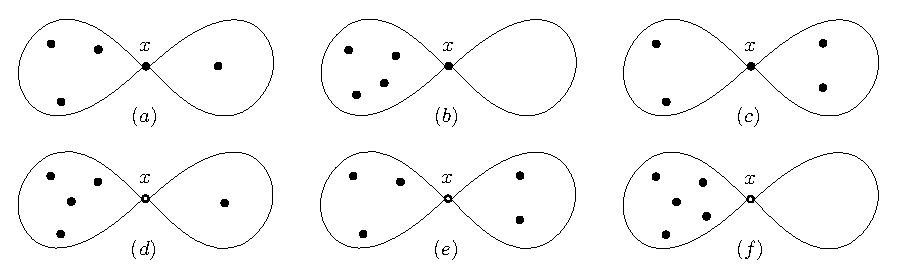
\includegraphics[width=13cm]{img/hourglass+1-cases.eps}
       \vspace{0.3cm}
       \caption{All cases of cut vertices in a 1-connected graph}
       \label{fig:2connected_counterexamples}
   \end{figure}
   
 Notice that for the cases (a), (b), and (c), the cut vertex $x$ is a transversal vertex.
   

   $H$ does not have a vertex of degree one, otherwise By Theorem \ref{thm:6}, we have that $K_4$ is $km$-forcing and $K_4 + 1$ vertex with degree one is also $km$-forcing (By Theorem \ref{thm:2}).
   Since if graph is $km$-forcing then all its subgraphs are also $km$-forcing (By Theorem \ref{thm:1}), then $H$ would be $km$-forcing, which is a contradiction.

 We have that all vertices in $H$ have degrees at least two, and if all of them are exactly two, then $H$ is a cycle, and By Theorem 4 in \cite{matthias_2022}, we have that
 all cycles are $km$-forcing, hence $H$ would be $km$-forcing, which is a contradiction.

 So we have that $H$ has at least one vertex of degree at least three; if it is exactly three and the rest are two, then by handshake lemma, we have at least 
 two vertices of degree three. If its' degree is four and the rest of the vertices have degree two, then we get that the graph $H$ is 
 the hourglass graph, which by Theorem \ref{thm:5} is $km$-forcing, hence $H$ would be $km$-forcing, which is a contradiction. So we have
 at least two vertices in $H$ that have a degree of at least three, and the rest have a degree of at least two.

 Let $R$ be the subgraph of the right side of the cut and $L$ be the subgraph of the left side of the cut.
 
 \begin{itemize}
    \item \textbf{Case (a)}: 
    Let us denote the transversal vertex in $R$ as $y$, and since 
 all vertices in $H$ have degrees at least two, then we have to have at least two Kempe chains between $y$ and two other transversal vertices in $G$. All paths from $y$ to other transversal vertices may only pass through
    $x$ because except $x$, all other transversals are in $L$; since $x$ is a transversal vertex itself, we can have a kempe chain from $y$ to $x$, but since $y$ and $x$ have different
 colors, we cannot have more Kempe chains going from $y$ through $x$ to other transversal vertices. Hence, we have only one Kempe chain from $y$ to other transversal vertices, bringing us to a contradiction.


    \item \textbf{Case (b)}: 
    Unlike case (a), we can realize all necessary Kempe chains. If no Kempe chain between transversals has edges in $R$, we can contract
 all vertices of $R$ into $x$ and preserve all Kempe chains between transversals; hence, $G$ was not a minimal graph, a contradiction.
 So let us assume there is some Kempe chain which has a subpath in $R$; since all Kempe chains start from $L$, such a Kempe chain has to pass through $x$; this means that if 
    $G$ is a counter-example; after contracting all edges of the $R$ into $x$, we still have left Kempe chains between all necessary transversals in $L$, but we got a smaller graph
 which still should be a counter-example; if the contracted version is not a counter-example, then it would mean $G$ was not a counter-example in the beginning since we could get a 
 rooted minor $H$ from G. Hence, the graph $G$ is not minimal, which is a contradiction.

    \item \textbf{Case (c)}: 
    If both vertices with degrees at least three are in $R$, let us denote them as $y, z$, then we can only have Kempe chains from $y$
 to $x$ and $z$, and from $z$ to $x$ and $y$, but $deg(y) >= 3, deg(z) >= 3$ in $H$, which is a contradiction since they can have 
 at most two Kempe chains in $G$ in this case. Then, assume only one vertex of degree, at least three, is in $R$, and let it be $y$. Similarly, we get that $y$ can have
 at most two Kempe chains, which is a contradiction. Symmetrically, the same holds if $x$ and $y$ were in $L$ or one of them was in $L$; hence, in all cases, we get a contradiction.

    \item \textbf{Case (d)}: 
    The vertex in $R$ has a degree of at least two. Hence, the color of $x$ is the color of the vertex itself,
so we can contract the paths from it to $x$ and still get the counter-example, which is a contradiction since the graph $G$ was not minimal.
    \item \textbf{Case (e)}:
    Let vertices in $L$ be denoted as $a,b,c$ and the vertices in $R$ as $y, z$, if we have at least one vertex with degree at least three in $R$, let it be $y$, then we can have
one Kempe chain between $y$ and $z$, and at least two Kempe chains from $y$ to $L$, hence $x$ has the color of $y$, but now since $z$ has 
degree at least two, at least one Kempe chain from $z$ should go to $L$, and it can pass only through $x$, since the color of $x$ is the same color as $y$, the 
Kempe chain from $z$, even if it includes $x$, can only be connected to $y$; hence, it cannot pass to $L$, which is a contradiction.
So we have that both vertices with degrees at least three are in $L$; in $L$ we have three vertices, and if all of them are maximally connected to each other, 
we get the $abc$ cycle, and since two vertices in $L$ have a degree of at least three, at least two Kempe chains should pass from $L$ to $R$, both of them pass through $x$, 
so both of them should be connected to the same transversal vertex in $R$, WLOG it is $y$, but then $z$ in $R$ can only be connected to $y$ if it has
Kempe chain to any other transversal than $y$, it has to pass through $x$ but $x$ has color of $y$, so the only Kempe chain from $z$ including $x$ can go to $y$
which is a contradiction since in $H$ $deg(z) >= 2$, we only can have one Kempe chain in $G$ from $z$
    \item \textbf{Case (f)}:
    We could contract all the vertices from $R$ into $x$ and still get the counter-example
    because all the Kempe chains still exist between the transversals, it contradicts the minimality of $G$.
 \end{itemize}
Thus, $G$ is 2-connected.
\end{proof}
\chapter{Computer Enumeration for Finding Counter-Examples in \( K_6 \)}

Since it remains open whether \( K_5 \) and \( K_6 \) are \( km \)-forcing, it is natural to attempt to find a counter-example.
A single counter-example would show that the graph is not \( km \)-forcing.
We performed a computer enumeration of the process of generating graphs \( G \) with a coloring \( \mathfrak{C} \) and a transversal \( T \) for a given minor \( H \),
where \( H \) is isomorphic to \( H(G, \mathfrak{C}, T) \). We then checked whether \( H \) is a rooted minor in \( G \).

The idea is similar to the previous chapter's construction of \( Z(G) \). 
We want to have all necessary Kempe chains between transversal vertices while ensuring that these vertices have no more than the necessary degrees.
However, since Kriesell and Mohr \cite{matthias_2022} showed that for every graph \( G \) with at most six vertices, the construction \( Z(G) \) does not
provide a counter-example \ref{thm:zg-for-k_6} (i.e., \( G \) remains a rooted minor of \( Z(G) \)), for looking for counter-examples 
for $K_6$, we must consider different constructions.

At a high level, our algorithm for finding possible counter-examples works as follows.
We begin with a given rooted minor \( H \) and construct a set of colorings.
The coloring is chosen so that the vertices of \( H \) are the transversals of those colorings; in other words, the transversal set corresponds to the vertex set of \( H \). 

Next, we construct graphs for each coloring where each edge of $H$ corresponds to a Kempe chain between the corresponding transversal vertices. After the Kempe chains are built, 
we know that \( H \) is the routing graph of all those graphs with their coloring and the transversal $V(H)$. 
Then, we check whether those graphs contain \( H \) as a rooted minor. 
If we find a graph \( G \) where \( H \) is not a rooted minor, we have found a counter-example.

The algorithm follows these three main steps:
\begin{enumerate}
    \item Given a graph \( H \), generate set of colorings such that the transversal \( T = V(H) \).
    \item For each such coloring, construct graphs $G$ where each edge of $H$ corresponds to a Kempe chain in $G$ between the transversal vertices.
    \item For each constructed graph \( G \), check whether \( G \) contains \( H \) as a rooted minor.
\end{enumerate}

\section{Step 1: Generating Colorings}
In the first step, we generate colorings, where each coloring has \(n\) vertices.

Each transversal of a coloring should be mapped to the vertices of $H$. Therefore, each coloring would have $|V(H)|$ colors.
First, we assign the colors to the transversal vertices and map them with $V(H)$, then for the rest of $n - |V(H)|$ vertices, we assign all possible combinations with the replacement of the colors  $1, \dots |V(H)|$ 

\begin{example}
 Let \(H = K_3\) (so \( |V(H)| = 3 \)) and let \(n = 8\). 
 First, we select three vertices and make them the transversals. We give each of them a distinct color from $1, 2, 3$.
 Then, we have $\binom{7}{3} = 35$ ways to assign colors for the five remaining vertices. Hence, we get 35 different colorings.
\end{example}


\begin{algorithm}[H]
    \caption{\textsc{GenerateColorings}$(H, n)$:}
    \label{alg:balanced-coloring}
    \begin{algorithmic}[1]
    \Require Graph $H$ all differently colored vertices, with $k = |V(H)|$, number of vertices $n$
    \Ensure Set of colorings $\mathcal{A}$

    \State Initialize empty coloring $\mathfrak{C} \gets \{\}$
    
    \For{each vertex $v \in V(H)$}
        \State Create new vertex $v'$
        \State Set $v'.isTransversal$ $\gets True$
        \State Set $v'.color$  $\gets v.color$
        \State Add $v'$ to $\mathfrak{C}$
    \EndFor
    

        \State $R \gets$ all combinations with replacement of $|V(H)|$ elements from $n - |V(H)|$
        \For{each combination $r \in R$}
            \State $\mathfrak{C}' \gets$ copy of $\mathfrak{C}$
            \For{each $v \in r$}
                \State Create new vertex $v'$
                \State Set $v'.isTransversal$ $\gets False$
                \State Set $v'.color$  $\gets v.color$
                \State Add $v'$ to $\mathfrak{C}'$
            \EndFor
            \State Add $\mathfrak{C}'$ to $\mathcal{A}$
        \EndFor
    
    \State \Return $\mathcal{A}$
    \end{algorithmic}
\end{algorithm}
    
\paragraph{Complexity Analysis.}
Let \( k = |V(H)| \) be the number of colors and \( n \) the number of vertices to generate.

\begin{itemize}
    \item In the beginning the algorithm creates $|V(H)|$ colors.
    
    \item Then we generate all combinations with replacement.
    \[
        \binom{k + n - 1}{k} \in \mathcal{O}(k^{n + k - 1})
    \]
    \item 
 For each combination, we create a new coloring, assuming the creation of the coloring,  
 creating a new vertex, and adding it to the coloring takes constant time. Creating a new coloring
 takes $\mathcal{O}(k)$ time.
    
    \item Overall, since the dominating step is the generation of all combinations with replacement, and for each such combination, 
 we use $\mathcal{O}(k)$ time to create a new coloring, we get the total time complexity \( \mathcal{O}(k^{n+k}) \).
\end{itemize}


\section{Step 2: Constructing Kempe Chains}

For each coloring $\mathfrak{C}$, we build graphs such that $H$ is the routing graph of those graphs. After finishing the construction of 
We check whether $H$ is a rooted minor in those graphs.

Below is an overview of the algorithm. At any point, we have a graph $G$ with all vertices colored and a list of remaining edge–pairs (chains) from $H$ to construct. For each edge $(s_i,t_i)$ from $E(H)$, we attempt to connect the corresponding $s_i$ to $t_i$ from $G$ by growing a Kempe chain:

\begin{itemize}
    \item Start at the current vertex $s_i$ and identify the next color needed (either that of $t_i$ or the current vertex if we have just matched $ t_i$'s color).
    \item Among all unvisited vertices of that color, pick one, add an edge to extend the chain, mark it visited, and recurse from this new vertex.
    \item Repeat until we reach $t_i$, at which point the chain for $(s_i,t_i)$ is complete.
\end{itemize}

Once one chain is complete, we move on to the next pair in the list. After all Kempe chains have been built, we perform a minor check (see Section~\ref{sec:check-minor}) to confirm that $H$ appears as a rooted minor of $G$.

\begin{algorithm}[H]
    \caption{\textproc{BuildKempeChains}$(G, \mathit{chains}, s, t, \mathit{visited}, \mathit{available}, H)$}
    \begin{algorithmic}[1]
        \Statex \textbf{Input:}
        \begin{itemize}
            \item $G$ — adjacency map of the graph
            \item $\mathit{chains}$ — list of pairs $(s_i,t_i)$ to connect
            \item $s$ — current chain start vertex
            \item $t$ — current chain end vertex
            \item $\mathit{visited}$ — set of vertices in the current chain
            \item $\mathit{available}$ — list of available vertices to extend chain
            \item $H$ — minor to test existence against
        \end{itemize}
        \Statex \textbf{Procedure:}
        \If{$s = t$}
            \If{$\mathit{chains} = \emptyset $}
                \If{\textproc{TestMinor}($H$, edges($G$))}
                    \Return
                \Else
                    \State \textbf{report counterexample}
                \EndIf
            \Else \Comment{Building new chain}
                \State $(s',t') \gets \mathit{chains.extract()}$
                \State $c \gets$ color($t'$)
                \State $\mathit{available} \gets \{v \in V(G): \text{color}(v)=c\}$
                \State \Call{BuildKempeChains}{$G,\mathit{chains},s',t',\{s'\},\mathit{available},M$}
            \EndIf
            \State \Return
        \EndIf

        \ForAll{$v \in \mathit{available}$}
            \State $G' \gets$ \textproc{copy}($G$)
            \State add edge $(s,v)$ in $G'$ 
            \State $c \gets \begin{cases}
 \text{color}(s), & \text{if } \text{color}(v) = \text{color}(t) \\
 \text{color}(t), & \text{otherwise}
            \end{cases}$
            \State $\mathit{visited}' \gets \mathit{visited} \cup \{v\}$
            \State $\mathit{available}' \gets \{ w \in V(G'): w \notin \mathit{visited}' \wedge \text{color}(w)=c\}$
            \State \Call{BuildKempeChains}{$G',\mathit{chains},v,t,\mathit{visited}',\mathit{available}',M,S$}
        \EndFor
    \end{algorithmic}
\end{algorithm}

\paragraph{Complexity Analysis.}

Let $n: = |V(G)|, m: = |E(H)|$

\begin{enumerate}
  \item \textbf{Single chain}
 At each recursive step, we choose at most \(n\!-\!1\) unvisited vertices of a single color and never revisit a vertex. Hence, we have recursion depth up to \(n\) in the worst case. So:
    \[
 \text{calls per chain}
 = 1 + (n-1) + (n-1)(n-2) + \cdots 
 = \mathcal{O}\bigl((n-1)!\bigr)
      \;=\; O(n!) 
    \]
  \item \textbf{All chains.}
 We build \(m\) chains, so overall we get.
    \[
      \mathcal{O}\bigl(m \cdot n!\bigr).
    \]
  \item \textbf{Minor check.}
 We will see in \ref{sec:check-minor} that testing for the rooted minor is done in \(\mathcal{O}(n_Hn_Ge_H(e_G + n_G\log{n_G}))\), where $n_G$ is the number of vertices of the larger graph, $n_H$ the number of vertices of the minor, and $e_H$ the number of edges of the minor. This runtime is 
 insignificant compared to $O(n!)$.
\end{enumerate}

Hence, the overall worst‑case time complexity is
\[
    \mathcal{O}\bigl(m \cdot n!\bigr).
\]


\section{Step 3: Checking for Rooted Minors}\label{sec:check-minor}
Finally, for each constructed graph~$G$, we check whether it contains~$H$ as a rooted minor. If any such~$G$ fails to contain~$H$, we have found a counter-example.

For this step, we use a heuristic tool for finding minor embeddings~\cite{dwavesystems2023minorminer}. The primary function we rely on is \texttt{find\_embedding()}, which implements the heuristic algorithm described in~\cite{cai2014practicalheuristicfindinggraph}.
Since \texttt{find\_embedding()} is a heuristic, we can be sure it exists when it returns an embedding of~$H$ in~$G$. However, when it returns no embedding, we cannot immediately conclude that one does not exist.

To reduce the false negatives, if no embedding is found, we rerun the function 10 additional times with different random seeds. While the authors of the algorithm do not provide an estimate for the probability of false negatives (returning no embedding when one exists) or any 
probabilistic quantity that we can rely on in our practice in most cases,
the function returns an embedding on the first try and succeeds within two or three retries.

The algorithm is the following:
\begin{algorithm}[H]
    \caption{TestIfMinorExists($H$, $G$, $S$)}
    \begin{algorithmic}[1]
        \Statex \textbf{Input:} 
        \begin{itemize}
            \item \( H \) — the target minor graph
            \item \( G \) — the parent graph to check
        \end{itemize}
        \Statex \textbf{Output:} True if $H$ is a rooted minor of $G$, otherwise False.

        \State $embedding \gets {find\_embedding}(H, G)$
        \If{$embedding \neq \emptyset$}
            \State \Return True
        \EndIf

        \For{$i \gets 1$ \textbf{to} 10}
            \State $seed \gets$ random integer
            \State $embedding \gets {find\_embedding}(H, G, \text{random\_seed} = seed)$
            \If{$embedding \neq \emptyset$}
                \State \Return True
            \EndIf
        \EndFor

        \State \Return False
    \end{algorithmic}
\end{algorithm}

\paragraph{Complexity Analysis.}

The \texttt{find\_embedding} function runs in
\[
  \mathcal{O}\bigl(n_H\,n_G\,e_H\,(e_G + n_G \log n_G)\bigr),
\]
as described in~\cite{cai2014practicalheuristicfindinggraph}, where $n_G$ is the number of vertices of the larger graph, $n_H$ the number of vertices of the minor, and $e_H$ the number of edges of the minor.

Since, in the worst case, we perform this operation 10 times, the total complexity still is:
\[
  \mathcal{O}\bigl(n_H\,n_G\,e_H\,(e_G + n_G \log n_G)\bigr).
\]

\section{Bringing everything together}
\label{main:algo:section}

We combine all the subroutines discussed in the previous paragraphs for the main algorithm. For a given rooted minor  
$H$ and a number of vertices $n$ in the parent graphs, we first generate all possible colorings for $n$ and $H$, where  
the transversal vertices of each coloring are mapped to the vertices of $H$. Then, for each such coloring, we build graphs consisting only  
of Kempe chains, such that there is a Kempe chain between two transversal vertices of the coloring if and only if those two transversals  
form an edge in $H$. After constructing all Kempe chains, we test whether $H$ is a rooted minor of that graph. If it is not a  
rooted minor, then we know that $H$ is non-$km$-forcing and that any graph such that $H$ is a subgraph of it is also non-$km$-forcing.

\begin{algorithm}[H]
    \caption{Searches for counter-examples}
    \label{alg:rooted_minor_search}
    \begin{algorithmic}[1]
      \Statex \textbf{Input:}
      \begin{itemize}
        \item $H$ — rooted minor we look for.
        \item $n$ — number of vertices in the parent graph $G$
      \end{itemize}
      \Statex \textbf{Output:} Graph $G$ where $H$ is a routing graph of $G$ with its corresponding coloring and transversal but not a rooted minor in $G$, or \textbf{None} if no such pair exists.
  
      \State $\textit{colorings} \gets \textsc{GenerateColorings}(H, n)$
      \ForAll{coloring $\mathfrak{C}$ \textbf{in} $\textit{colorings}$}
        \State $G \gets$ empty graph on $\mathfrak{C}$
        \State $result \gets \textsc{BuildKempeChains}(G, E(H), s, t, \emptyset, \mathit{available}, H)$
        \If{$result \neq \textbf{None}$}
          \State \Return $result$ \Comment{Found a counter-example}
        \EndIf
      \EndFor
  
      \State \Return \textbf{None} \Comment{No counter-examples found}
    \end{algorithmic}
  \end{algorithm}

\paragraph{Complexity Analysis.}
Let $k$ = $|V(H)|$, let $m$ = $|E(H)|$.
\begin{enumerate}
    \item \textsc{GenerateColorings} takes $\mathcal{O}(k^{n+k})$ time
    \item We have $\mathcal{O}(k^{n+k})$ colorings and for each coloring \textsc{BuildKempeChains} takes $\mathcal{O}\bigl(m \cdot n!\bigr)$ time.
 So overall the main for loop takes $\mathcal{O}\bigl(k^{n+k} \cdot m \cdot n!\bigr)$ time
\end{enumerate}

Since the main loop dominates the time complexity, we get the overall time complexity of the algorithm as follows:

\[
    \mathcal{O}\bigl(k^{n+k} \cdot m \cdot n!\bigr)
\]

\section{Results}

First, with the subroutine \textsc{TestIfMinorExists}, we verified the result of \cite{matthias_2022} that $K_7$ is non-$km$-forcing.

We used the main algorithm from \ref{main:algo:section} to primarily test whether $K_6$ is non-$km$-forcing or not.  
By \ref{thm:1}, finding any non-$km$-forcing subgraph of $K_6$ is sufficient to prove that $K_6$ is non-$km$-forcing.  
Since we also know that $K_4$ is $km$-forcing \ref{thm:3} and that graphs with five vertices and at most six edges are $km$-forcing,  
the subgraphs of $K_6$ we are looking for are in between dense graphs on five vertices and graphs on six vertices.  
Moreover, we know that all cycles are $km$-forcing \ref{thm:4}, so we do not need to consider $C_6$.  
Adding a pending edge to a $km$-forcing graph still keeps this property \ref{thm:2}.  
So, we have a limited amount of subgraphs of $K_6$ to consider.

Because the algorithm has super-exponential time complexity, we could test for all candidate subgraphs of $K_6$  
We found no counter-examples on parent graphs with at most 13 vertices.
\chapter*{Conclusion}
\addcontentsline{toc}{chapter}{Conclusion}

In this thesis, we surveyed the results of Hadwiger's conjecture and Kempe chains, focusing on Kriesell and Mohr's results. 
We have worked on computer-assisted graph enumeration to search for counterexamples for $K_6$ to show that it is non-KM-forced in some graph $G$ but found no counterexamples in graphs up to 13 vertices.
We believe that there are counterexamples for $K_6$, but they are larger than 13 vertices, so to find them, 
we would need to use more computational power or a better algorithm. Furthermore, we showed that any minimal counterexample $G$ such that $K_5$ is non-KM-forced in $G$, 
must be 2-connected, which might be a step towards proving the case $k=5$.

%%% Bibliography
%%% Bibliography (literature used as a source)
%%%
%%% We employ biblatex to construct the bibliography. It processes
%%% citations in the text (e.g., the \cite{...} macro) and looks up
%%% relevant entries in the bibliography.bib file.
%%%
%%% See also biblatex settings in thesis.tex.

%%% Generate the bibliography. Beware that if you cited no works,
%%% the empty list will be omitted completely.

% We let bibliography items stick out of the right margin a little
\def\bibfont{\hfuzz=2pt}

\printbibliography[heading=bibintoc]

%%% If case you prefer to write the bibliography manually (without biblatex),
%%% you can use the following. Please follow the ISO 690 standard and
%%% citation conventions of your field of research.

\begin{thebibliography}{99}

\bibitem{lamport94}
  {\sc Lamport,} Leslie.
  \emph{\LaTeX: A Document Preparation System}.
  2nd edition.
  Massachusetts: Addison Wesley, 1994.
  ISBN 0-201-52983-1.

\end{thebibliography}


%%% Figures used in the thesis (consider if this is needed)
\listoffigures

%%% Tables used in the thesis (consider if this is needed)
%%% In mathematical theses, it could be better to move the list of tables to the beginning of the thesis.
% \listoftables

%%% Abbreviations used in the thesis, if any, including their explanation
%%% In mathematical theses, it could be better to move the list of abbreviations to the beginning of the thesis.
% \chapwithtoc{List of Abbreviations}

%%% Doctoral theses must contain a list of author's publications
\ifx\ThesisType\TypePhD
\chapwithtoc{List of Publications}
\fi

%%% Attachments to the thesis, if any. Each attachment must be referred to
%%% at least once from the text of the thesis. Attachments are numbered.
%%%
%%% The printed version should preferably contain attachments, which can be
%%% read (additional tables and charts, supplementary text, examples of
%%% program output, etc.). The electronic version is more suited for attachments
%%% which will likely be used in an electronic form rather than read (program
%%% source code, data files, interactive charts, etc.). Electronic attachments
%%% should be uploaded to SIS. Allowed file formats are specified in provision
%%% of the rector no. 72/2017. Exceptions can be approved by faculty's coordinator.
\appendix
\chapter{Attachments}

\section{First Attachment}

\end{document}
